% vim: set foldmethod=marker foldlevel=0:

\documentclass[a4paper, 11pt]{article}
\usepackage[UKenglish]{babel}

\usepackage[margin=2.4cm]{geometry}

\usepackage[hidelinks]{hyperref}

\usepackage{preamble}

\usepackage{tikz}

\renewcommand{\thesubsection}{\hspace*{-2.75em} (\alph{subsection})}

\fancyhead[L]{CS260 Assignment 2}
\title{CS260 Algorithms, Assignment 2}
\colorlet{questionbodycolor}{yellow!50!pink}

\begin{document}

% TODO: Comment out the question body before submitting

% Question body {{{

\maketitle

\setlength{\parindent}{0em}
\setlength{\parskip}{1em}

\fancyhead[C]{}

\pagenumbering{roman}

\question{1}

\begin{questionbody}
The Daventry Heritage Railway is planning out its winter season, and would like to run a special Santa Service to encourage more people to visit the picturesque local area during the winter time.

The Railway has stops arranged as in Figure~\ref{fig:railway-map-graph}.

In order to run their Santa Service, they need to plot a route that visits all stations on the Railway. The route should not pass through any station twice, EXCEPT at the end of the line, where they need to pass through two stops and loop back to a third, so the train can now go back the other way.

A Santa Service therefore comprises two parts: a \textit{route} comprising all but 2 stops; and a cycle of size 3, which is the \textit{reversing loop}, meeting one end of that route and including the other 2 stops.
\begin{enumerate}[(a)]
\item Can Daventry Heritage Railway set up a Santa Service based on their current rail map?
\end{enumerate}

Let \textsc{Santa-Service} be the problem of determining, for a given map (provided as an undirected graph), whether a Santa Service exists.
\begin{enumerate}[(a), start=2]
\item Give an algorithm for \textsc{Santa-Service}.

\item Show that \textsc{Santa-Service} is complete for NP\@.

\item Let the \textsc{Find-Santa-Service} problem be the equivalent problem where we \textbf{return} a valid Santa Service (or nothing) instead of only returning whether one exists. Is \textsc{Find-Santa-Service} in NP\@? Is it NP-hard? Is it NP-complete?

\item Give a restriction of the input under which \textsc{Santa-Service} is solvable in polynomial time, but not in constant time.
\end{enumerate}

\textit{Note}: For \textbf{ALL} parts of this assignment, you are expected to justify that your answer is correct with an appropriate argument or full proof. Answers without an attempt at justification will not be rewarded.
\end{questionbody}

\begin{figure}[tbhp]
\centering

\begin{minipage}{0.4\linewidth}
\centering
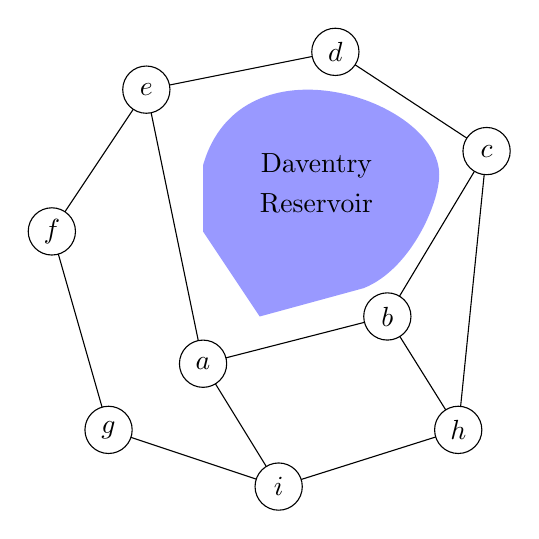
\begin{tikzpicture}[scale=1.2]
    \coordinate (a) at (1.8, 1.5);
    \coordinate (b) at (3.75, 2);
    \coordinate (c) at (4.8, 3.75);
    \coordinate (d) at (3.2, 4.8);
    \coordinate (e) at (1.2, 4.4);
    \coordinate (f) at (0.2, 2.9);
    \coordinate (g) at (0.8, 0.8);
    \coordinate (h) at (4.5, 0.8);
    \coordinate (i) at (2.6, 0.2);

    \draw (a) -- (b);
    \draw (a) -- (e);
    \draw (a) -- (i);
    \draw (b) -- (c);
    \draw (b) -- (h);
    \draw (c) -- (d);
    \draw (c) -- (h);
    \draw (d) -- (e);
    \draw (e) -- (f);
    \draw (f) -- (g);
    \draw (g) -- (i);
    \draw (i) -- (h);

    \draw[fill=white] (a) circle[radius=0.25];
    \draw[fill=white] (b) circle[radius=0.25];
    \draw[fill=white] (c) circle[radius=0.25];
    \draw[fill=white] (d) circle[radius=0.25];
    \draw[fill=white] (e) circle[radius=0.25];
    \draw[fill=white] (f) circle[radius=0.25];
    \draw[fill=white] (g) circle[radius=0.25];
    \draw[fill=white] (h) circle[radius=0.25];
    \draw[fill=white] (i) circle[radius=0.25];

    \node () at (a) {$a$};
    \node () at (b) {$b$};
    \node () at (c) {$c$};
    \node () at (d) {$d$};
    \node () at (e) {$e$};
    \node () at (f) {$f$};
    \node () at (g) {$g$};
    \node () at (h) {$h$};
    \node () at (i) {$i$};

    \fill[blue!40] (2.4, 2)
        -- (1.8, 2.9)
        -- (1.8, 3.6)
        .. controls (2.2, 5) and (4.3, 4.3) .. (4.3, 3.5)
        .. controls (4.3, 3.2) and (4, 2.5) .. (3.5, 2.3)
        -- cycle;

    \node () at (3, 3.6) {Daventry};
    \node () at (3, 3.2) {Reservoir};
\end{tikzpicture}
\end{minipage}\hspace{3em}
%
\begin{minipage}{0.4\linewidth}
\begin{tabular}{c|l} % chktex 44
    \textbf{Stop} & \textbf{Name} \\
    $a$ & Anglers' Nook \\
    $b$ & Beach \\
    $c$ & Cedar Lodge \\
    $d$ & Daventry Reservoir North \\
    $e$ & Elm Lane \\
    $f$ & Football Fields \\
    $g$ & Groudle Glen \\
    $h$ & Headlands \\
    $i$ & Ice Town
\end{tabular}
\end{minipage}

\caption{Daventry Heritage Railway’s Christmas Map}\label{fig:railway-map-graph}
\end{figure}

\newpage
\pagenumbering{arabic}

% }}}

\setlength{\parindent}{0em}
\setlength{\parskip}{1em}

\fancyhead[C]{Page \thepage~of~\pageref*{last-page}}

\subsection{~} % a
\vspace*{-6.5ex}

Answer

\subsection{~} % b
\vspace*{-6.5ex}

Answer

\subsection{~} % c
\vspace*{-6.5ex}

Answer

\subsection{~} % d
\vspace*{-6.5ex}

\textsc{Find-Santa-Service} is not a decision problem so cannot be in NP and therefore cannot be NP-complete.
% TODO: Is it NP-hard?

\subsection{~} % e
\vspace*{-6.5ex}

Answer

\label{last-page} % chktex 24

\end{document}
